Models are a simplified mathematical description that captures some relevant physics of more complicated systems. This section introduces some specific models, their relevance and some properties. These models will be used later to benchmark the developed \Gls{TN} cluster expansions.

\subsection{Ising model}\label{models:ising}

The prototypical example of a model in the field of strongly correlated matter is the Ising model. It was first introduced 1925 by Ernest Ising, as a model to capture ferromagnetism. He proved that for a linear chain, there is no phase transition at finite temperatures. He wrongly concluded that this would also be the case in higher dimensions, but it turned out to be one of the deepest and far-reaching problems in the $20^{th}$ century \cite{Taroni2015}.

The Ising model, in essence, assigns an energy contribution to neighbouring spins. These spins sit on a fixed position on a chain (1D) or lattice (2D/3D/...). In classical Ising, the operators in the Hamiltonian all commute with each other. An energy is assigned between neighbouring spins. There is also a contribution for the alignment with an external magnetic field in the same direction. In \Gls{TFI} model, a transversal field is added. The operator measuring the transversal field no longer commutes with the operator measuring the alignment, and hence this is a quantum model. Often, the particles on the grid are spin 1/2 particles, but of course other particles are possible. Many generalizations exist for the Ising model, which will not be discussed her.

\subsubsection{Classical Ising}

The classical Ising model is given by the Hamiltonian
\begin{equation}
    H = -J \left (  \sum_{\Braket{i j }} \sigma_i \sigma_j + h \sum_i \sigma_i \right ),
\end{equation}
where $  \Braket{i j }$ runs over all neighbouring lattice sites. The possible values of $\sigma$ depends on the spin dimension. For spin $1/2$ lattices $\sigma \in {-1,+1}$. g encodes the interaction strength of the external magnetic field. The sign J determines the low temperature ground state. A positive J will tend to align all neighbouring spins at low temperature. This is often called ferromagnetic, because all the aligned spins cause a macroscopic magnetisation. On the other hand, a negative J causes neighbouring spins to have an opposite sign. Depending on the sign of the longitudinal field h, the spins tend to align or antialign with this external field. This lifts the degeneracy of the ground state.

\paragraph{1D}

The classical 1D model was solved analytically by Lens. It can be solved analytically and shows no phase transitions  at finite temperature.

\paragraph{2D}

In 2D, it becomes important to define the lattice. Here, and in the simulations, we will consider a square lattice. This model was famously solved by Lars Onsager in 1944, by using the transfer matrix method. In 2 dimensions, the Ising model has a continuous phase transition at finite temperature. The critical temperature is $T_c = \frac{2 J}{T ln( \sqrt{2}+1)}$. Only the $h=0$ case is solved analytically. For higher dimensions, no analytical solution is known. On different lattices, interesting things can happen. For instance, the ground state of an antiferromagnet on a triangular lattice is not obvious to determine. The spins tend to antialign, but at least 2 of 3 spins on the corner of a triangle have to align. This is called frustration.

\subsubsection{Transverse Field Ising}

As we all know, the real world behaves, certainly at small length and time scales, quantum mechanically. Therefore, it is important to understand how the \acrfull{TFI} model differs from the classical model. In the \Gls{TFI} model, the operators no longer commute with each other. An example is the \Gls{TFI} model given by the  Hamiltonian
\begin{equation}
    \hat{H} = -J \left (  \sum_{\Braket{i j }} \sigma^x_i \sigma^x_j + g \sum_i \sigma^z_i \right ) .
\end{equation}
In the case that $g=0$, this is the classical Ising model (in the $h=0$ case).

\paragraph{1D}
Different to the classical case, the 1D model contains a quantum phase transition at $g=1$. For smaller fields, the ground state has a macroscopic magnetisation, for higher g not. The transition is of type \Cref{fig:crit:qtran} (a). The critical value can be calculated exactly using the Kramers-Wannier duality \cite{Radicevic2018}. The fact that this model has a phase transition can also be understood with \cref{q2cmap}.

\paragraph{2D}

The 2D phase diagram of the \Gls{TFI} model is shown in \cref{2dtisingphasediag}. The notation $\Gamma=g$ is taken in this figure. The classical phase transition is visible at $g=0$. The red dot is the quantum critical point, situated at $ G \approx 3.04  $. A part of this phase diagram will be reproduced in \cref{subsec:qphasediag}.

\begin{figure}[!htbp]
    \center
    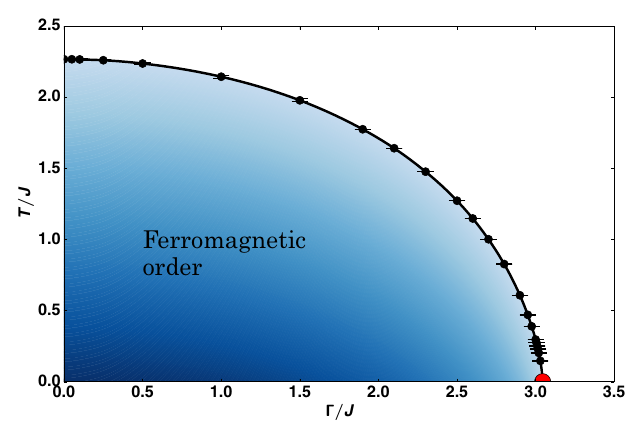
\includegraphics[width=\textwidth]{Figuren/phsyics/2disingphase.png}
    \caption{Phase diagram for 2D \Gls{TFI} model. Figure taken from \cite{Hesselmann2016}.}
    \label{2dtisingphasediag}
\end{figure}

\subsection{Heisenberg}

The Heisenberg model is given by
\begin{equation}
    \hat{H} =  -\left( \sum_{\Braket{i j }} J_x \sigma^z_i \sigma^z_j + J_y \sigma^y_i \sigma^y_j+ J_z \sigma^z_i \sigma^z_j + h \sum_i \sigma^z_i \right ).
\end{equation}
This is a whole class of models, and they have different names depending on the values of $J_{\alpha} $ with $\alpha=x,y,z$. E.g. $J_x = J_y \neq J_z = \Delta$ is called the XXZ model, because the weight for $\sigma^z$ is different. The isotropic version or simply Heisenberg model in the remainder of this thesis, which will be simulated in \cref{chap:results}. The model is
\begin{equation}
    \hat{H} =  -J \left( \sum_{\Braket{i j }} \vec{\sigma} \cdot \vec{\sigma} \right ).
\end{equation}

\subsection{Random}\label{randhamexpl}
It's also possible to construct random Hamiltonians. This is a useful, because it ensures that no special simple structure is present. The single site (which can be thought of as an external field as before) and nearest neighbour Hamiltonians are generated by making Hermitian matrices with random real and complex numbers between -1 and 1. In order to make them comparable, the energy scale is set such that the norm of the Hamiltonian evaluated on 2 sites is 1.

\subsection{Quantum to classical mapping}\label{q2cmap}

In a certain sense, a quantum model in d dimensions can be mapped to a classical model in d+1 dimension. Due to the Lie product formula
\begin{equation}
    e^{A+B} = \lim_{M \to \infty } ( e^{A/M} e^{B/M}  )^M
\end{equation}
we can rewrite the partition function as
\begin{equation}
    \begin{split}
        Z &= \sum_n e^{ - \beta E_n} \\
        &= \sum_n \Braket{n | e^{ - \beta \hat{H} }  | n} \\
        &= \sum_{n_1 \cdots n_M} \Braket{n_1 | e^{ - \beta \hat{H} /M}  | n_2}  \Braket{n_2 | e^{ - \beta \hat{H} /M }  | n_3} \cdots  \Braket{n_{M} | e^{ - \beta \hat{H} /M }  | n_1} \\
        &= \sum_{  n_1 \cdots n_M} \Braket{n_1 | e^{ - \beta \hat{H} /M}  | n_2}  \Braket{n_2 | e^{ - \beta \hat{H} /M }  | n_3} \cdots  \Braket{n_{M} | e^{ - \beta \hat{H} /M }  | n_1} \\
    \end{split}
\end{equation}
where completeness relations $ I = \sum_{n_i}  \ket{ n_i } \bra{ n_i}  $ inserted M times in line 3. This is similar to a path integral. The quantum imaginary time has become a spatial dimension. The quantum model of d dimensions now has the structure of a classical model in d+1 dimensions. In this way, the 2D \Gls{TFI} model can be mapped to the 3D classical Ising model \cite{Hsieh}.